
\documentclass[11pt]{article}
\usepackage{amsmath}
\usepackage{graphicx}

\begin{document}
\setcounter{page}{23}
\title{Appendix}
\date{\vspace{-5ex}}
\maketitle{}

Note that all of these models below were fit to each of the multiply imputed datasets, and the results are combined as discussed in the paper. All statistics below represent these combined results.

\section{Relationship}
I here present the extended methodology for the relationship analysis, as well as the results of the regression analysis.

\subsection{Simple relationship}
The simple relationship between various predictors and high school graduation was modeled as

\vspace{5mm}
$ logit(\pi) = \beta_0 + \beta_1(X) + \epsilon, $
\vspace{5mm}

\noindent where

\begin{itemize} \itemsep1pt \parskip0pt \parsep0pt
	\item $\pi$ is the probability of graduation from high school,
	\item $X$ is the variable of interest,
	\item and $\epsilon$ is an error term (for the sake of brevity, this is the only time I will mention this term).
\end{itemize}

\subsection{Controlled relationship}
I then modified the regression model to incorporate important potentially confounding covariates:

\vspace{5mm}
$ logit(\pi) = \beta_0 + \beta_1(sex) + \beta_2(race) + \beta_3(income) + \beta_4(familyEduc) + \beta_5(householdStructure)+ \beta_6(noncognitive) + \epsilon, $
\vspace{5mm}

\noindent where

\begin{itemize} \itemsep1pt \parskip0pt \parsep0pt
	\item $\pi$ is the probability of graduation from high school,
	\item $sex$ is a binary variable ($1=male, 2=female$) indicating the biological sex of the child, and
	\item $race$ is a categorical variable indicating the reported race of the child,
	\item $income$ is size-adjusted household income, smoothed available data between 1994 and 2001,
	\item $familyEd$ is a binary variable denoting the biological mother's high school graduations status,
	\item $householdStructure$ is a categorical variable denoting the presence of biological family in the home (larger is worse),
	\item and $noncognitive$ is the noncognitive score, computed as described in the study.
\end{itemize}

From here on, denote the vector of demographic covariates described above (everything except for $noncognitive$) $\mathbf{X}$.

\subsection{Full Results}
The full results are summarized in the table below.

{\centering
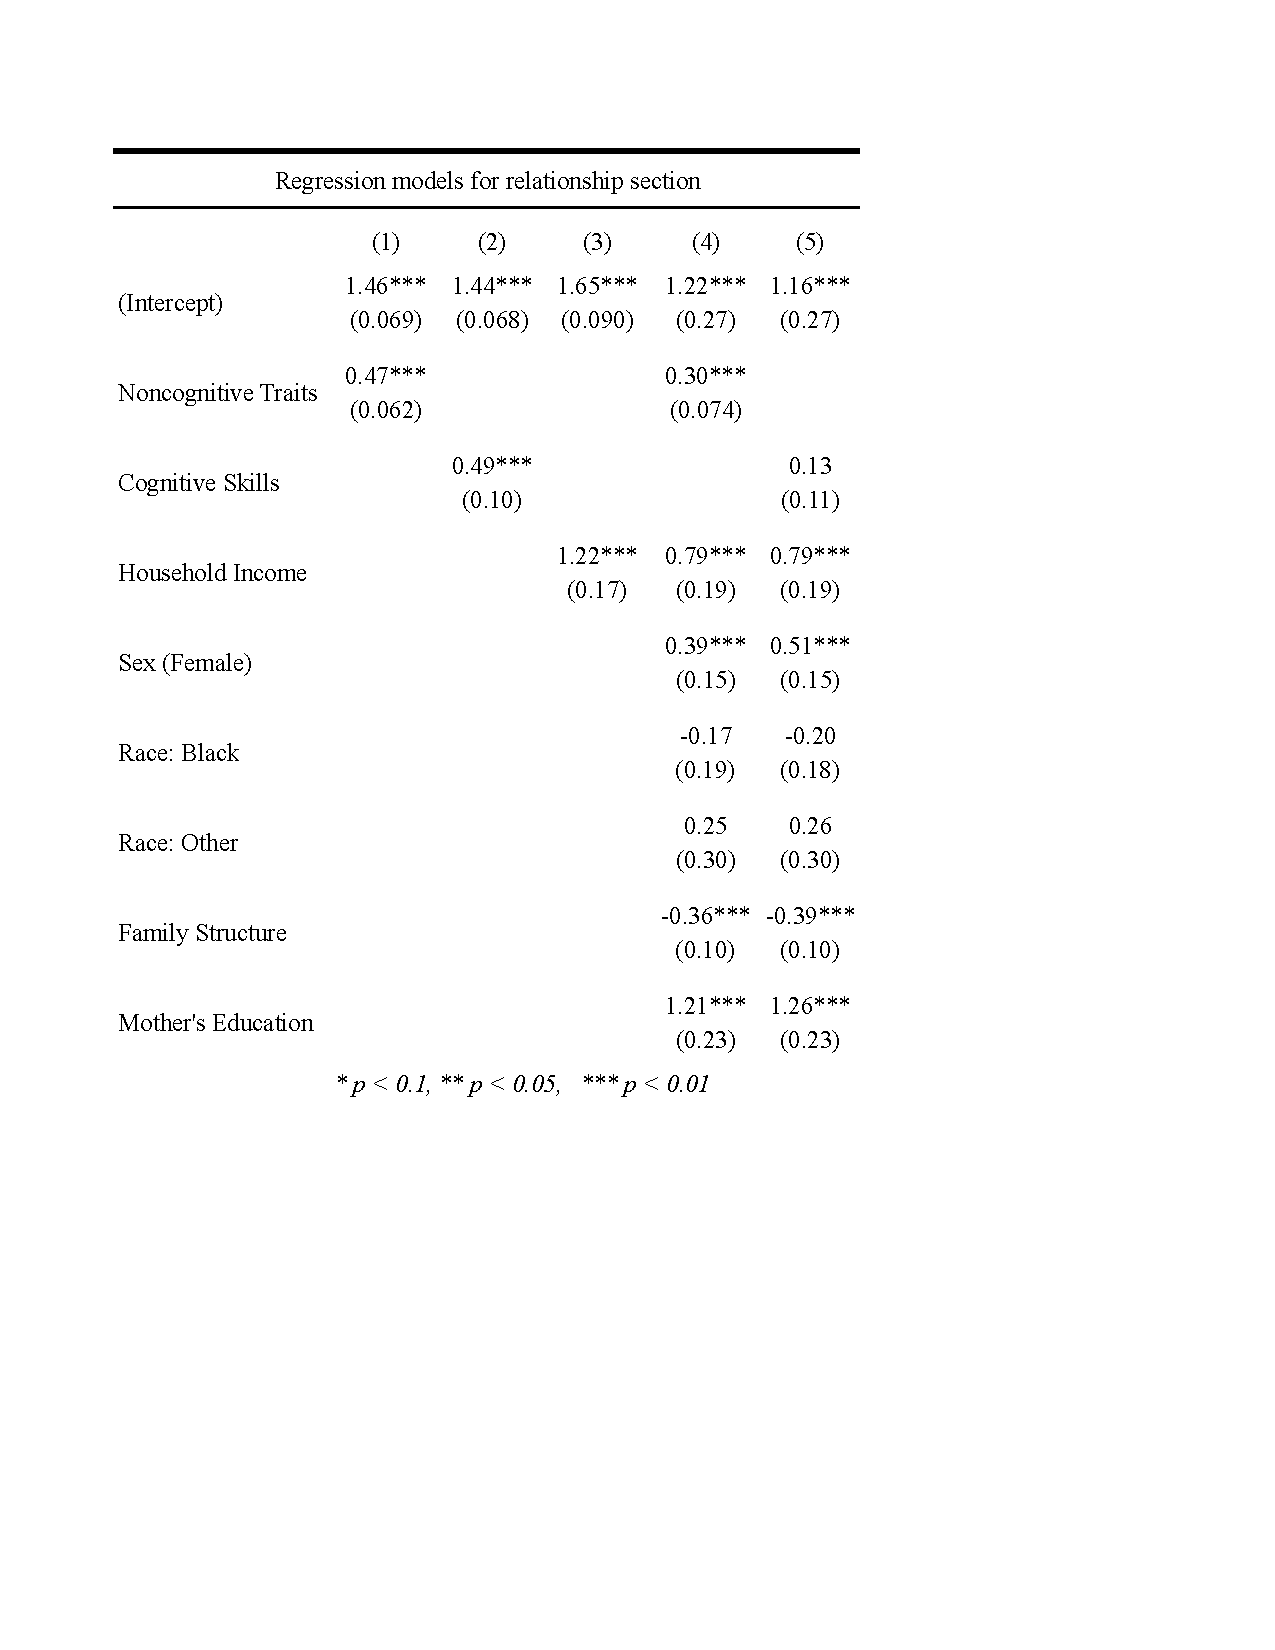
\includegraphics[scale=0.8]{relationship.pdf}\\}

\section{Mediation}
I here present extended methodological details for the mediation analysis. The simple path analysis involved fitting two models: 
\begin{itemize}\itemsep1pt \parskip0pt \parsep0pt
	\item noncognitive traits and demographic controls are used to predict the mediating factor
	\item noncognitive traits, demographic controls, and the mediating factor are used to predict the outcome (high school graduation).
\end{itemize}

As I mention in the main article, because of the flexibility needed in this particular case and the computation concerns introduced by the imputation, I opted to use a bootstrap-based estimation method implemented in R. As such, I do not present parameter estimates for the fitted models of the individual regressions.

The general models were as follows. For predicting the behavioral measures as mediating variables,

\vspace{5mm}
$log(E(b)) = \beta_0 + \boldsymbol{\beta}(\mathbf{X})+ \beta_n(noncognitive)+\epsilon,$
\vspace{5mm}

\noindent where

\begin{itemize}\itemsep1pt \parskip0pt \parsep0pt
	\item $log(E(b))$ is the log of the expectation of the count of event $b$ (problematic school behavior),
	\item $\mathbf{X}$ is the vector of demographic controls,
	\item and $noncognitive$ is the noncognitive score.
\end{itemize}

Again, this is modeled as Poisson. For predicting academic performance as the mediating variable, the model is simpler:

\vspace{5mm}
$gpa = \beta_0 + \boldsymbol{\beta}(\mathbf{X})+ \beta_n(noncognitive)+\epsilon,$
\vspace{5mm}

\noindent where
\begin{itemize}\itemsep1pt \parskip0pt \parsep0pt
	\item gpa is high school GPA,
	\item $\mathbf{X}$ is the vector of demographic controls,
	\item and $noncognitive$ is the noncognitive score.
\end{itemize}

For both of these models, the model for predicting the outcome was as follows:

\vspace{5mm}
$logit(\pi) = \beta_0 + \boldsymbol{\beta}(\mathbf{X})+ \beta_{n-1}(mediator) + \beta_{n}(noncognitive)+\epsilon,$
\vspace{5mm}

\noindent where
\begin{itemize}\itemsep1pt \parskip0pt \parsep0pt
	\item $\pi$ is the probability of graduating from high school,
	\item $\mathbf{X}$ is the vector of demographic controls,
	\item $mediator$ is the mediator being analyzed, either counts of misbehavior or GPA,
	\item and $noncognitive$ is the noncognitive score.
\end{itemize}

\section{Decomposition}
As mentioned in the study, I used two strategies for decomposition: interaction terms and separate regressions.

\subsection{Interaction terms}
For the interaction terms, the following model was used:

\vspace{5mm}
$logit(\pi) = \beta_0 + \boldsymbol{\beta}(\mathbf{X}) + \beta_{n-1} (noncognitive) +\beta_n(noncognitive*f) + \epsilon$
\vspace{5mm}

\noindent where

\begin{itemize}\itemsep1pt \parskip0pt \parsep0pt
	\item $\pi$ is the probability of graduation from high school, and
	\item $\mathbf{X}$ is the vector of demographic covariates described above, and
	\item $noncognitive$ is the noncognitive score, and
	\item $f$ is the factor of interest (one of the measures in $\mathbf{X}$)
\end{itemize}

The results of these models are presented in the table below.

{\centering
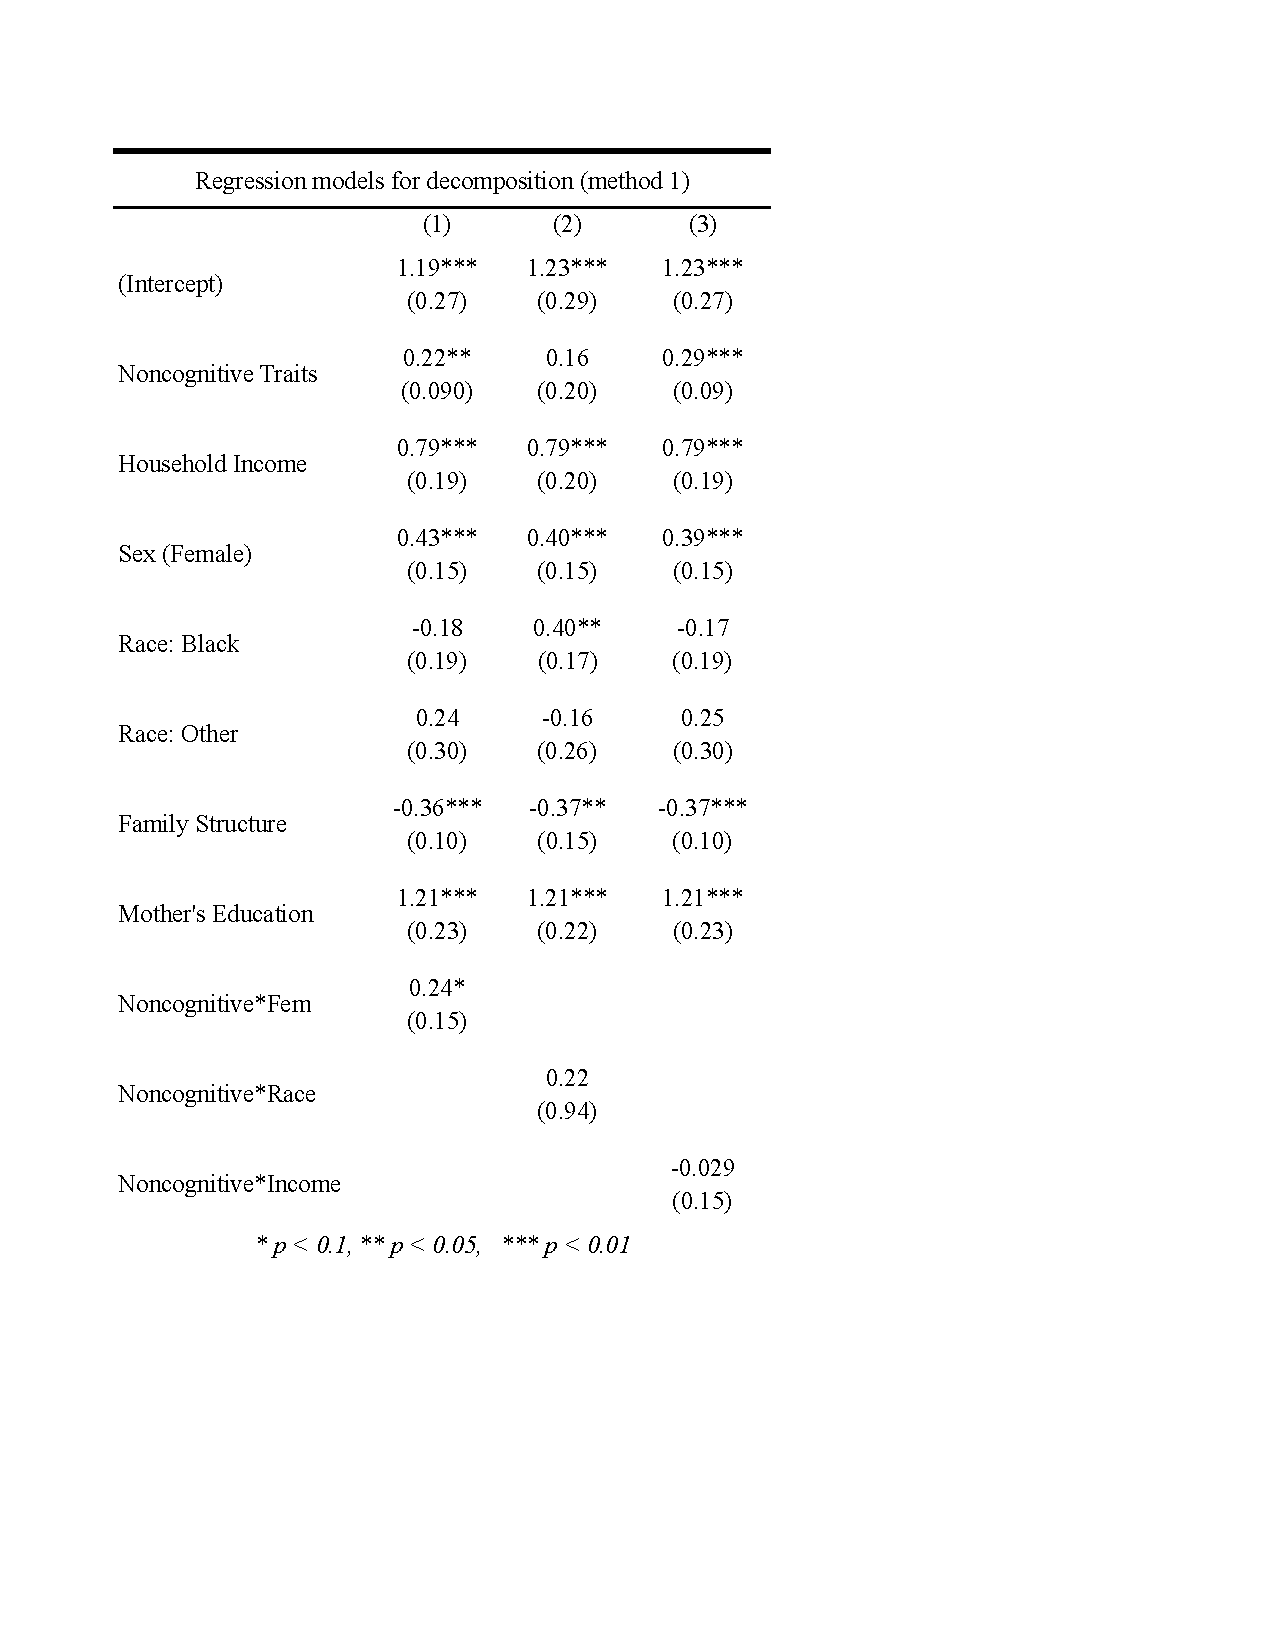
\includegraphics[scale=0.8]{decomp1.pdf}\\}

\subsection{Separate regressions}
For the separate regressions, the following model systems were estimated:

\vspace{5mm}
$logit(\pi) = \beta_0 + \boldsymbol{\beta}(\mathbf{X^-}_{group1}) + \beta_{n}(noncognitive_{group1}) + \epsilon$

\noindent and

$logit(\pi) = \beta_0 + \boldsymbol{\beta}(\mathbf{X^-}_{group2}) + \beta_{n} (noncognitive_{group2}) + \epsilon,$

\vspace{5mm}

\noindent where
\begin{itemize}\itemsep1pt \parskip0pt \parsep0pt
	\item $\pi$ is the probability of graduation from high school, and
	\item $\mathbf{X^-}$ is the vector of demographic characteristics, without the entry for the groups analyzed by each model, and
	\item $group$ designates the subset of entries upon which the model is run.
\end{itemize}

Note that I did not analyze using this strategy, as it is not necessarily logical to split it into discrete groups. Although I could have fit the statistically equivalent model with all of the interaction terms between income and the other variables, on the basis of the lackluster from the previous analysis, I decided to forgo this option.

For efficiency, the results of this approach is presented in the body of the text.

\end{document}